% ****** Start of file apssamp.tex ******
%
%   This file is part of the APS files in the REVTeX 4.2 distribution.
%   Version 4.2a of REVTeX, December 2014
%
%   Copyright (c) 2014 The American Physical Society.
%
%   See the REVTeX 4 README file for restrictions and more information.
%
% TeX'ing this file requires that you have AMS-LaTeX 2.0 installed
% as well as the rest of the prerequisites for REVTeX 4.2
%
% See the REVTeX 4 README file
% It also requires running BibTeX. The commands are as follows:
%
%  1)  latex apssamp.tex
%  2)  bibtex apssamp
%  3)  latex apssamp.tex
%  4)  latex apssamp.tex
%
\documentclass[
reprint,
%superscriptaddress,
%groupedaddress,
%unsortedaddress,
%runinaddress,
%frontmatterverbose, 
%preprint,
%preprintnumbers,
nofootinbib,
%nobibnotes,
%bibnotes,
amsmath, amssymb,
aps,
%pra,
%prb,
%rmp,
%prstab,
%prstper,
floatfix,
]{revtex4-2}

\bibliographystyle{apsrev4-2}

\usepackage{graphicx}% Include figure files
\usepackage{dcolumn}% Align table columns on decimal point
\usepackage{bm}% bold math
\usepackage{float}
% \usepackage{subcaption}% Subcaption for figures
\usepackage[T1]{fontenc}
\usepackage[utf8]{inputenc}
\usepackage{babel}
\usepackage{xcolor}
\usepackage{ulem}
%\usepackage{hyperref}% add hypertext capabilities
%\usepackage[mathlines]{lineno}% Enable numbering of text and display math
%\linenumbers\relax % Commence numbering lines

%\usepackage[showframe,%Uncomment any one of the following lines to test 
%%scale=0.7, marginratio={1:1, 2:3}, ignoreall,% default settings
%%text={7in,10in},centering,
%%margin=1.5in,
%%total={6.5in,8.75in}, top=1.2in, left=0.9in, includefoot,
%%height=10in,a5paper,hmargin={3cm,0.8in},
%]{geometry}

\begin{document}

\preprint{APS/123-QED}

\title{Liquid Xenon Positron Target}% Force line breaks with \\
% \thanks{A footnote to the article title}%

\author{Max Varverakis}
\email{mvarvera@calpoly.edu}
\affiliation{California Polytechnic State University, San Luis Obispo, CA 93407, USA}
\author{Spencer Gessner}%
\email{sgess@slac.stanford.edu}
\affiliation{SLAC National Accelerator Laboratory, Menlo Park, California 94025, USA}%

\author{Robert Holtzapple}
\email{rholtzap@calpoly.edu}
\affiliation{California Polytechnic State University, San Luis Obispo, CA 93407, USA}

\author{Hiroki Fujii}
\email{hiroki.fujii@riken.jp}
\affiliation{Nishina Center, RIKEN, 2-1 Hirosawa, Wako, Saitama, 351-0198, Japan}

% \collaboration{MUSO Collaboration}%\noaffiliation

% \author{Charlie Author}
%  \homepage{http://www.Second.institution.edu/~Charlie.Author}
% \affiliation{
%  Second institution and/or address\\
%  This line break forced% with \\
% }%
% \affiliation{
%  Third institution, the second for Charlie Author
% }%
% \author{Delta Author}
% \affiliation{%
%  Authors' institution and/or address\\
%  This line break forced with \textbackslash\textbackslash
% }%

% \collaboration{CLEO Collaboration}%\noaffiliation

\date{\today}

\begin{abstract}
Positron targets are a critical component of future linear colliders.
%Colliding high energy electrons with a high-Z material -- known as a positron target -- is a common method for producing positrons for particle accelerator applications.
Traditional targets are composed of high-Z metals that become brittle over time due to constant bombardment by high-power electron beams.
%The main consequence of using a solid positron target involves material degradation due to energy deposition from the beam, in which preventative measures require various techniques to dissipate thermal gains in the material.
We explore the possibility of a liquid Xenon target which is constantly refreshed and therefore not susceptible to the damage mechanisms of traditional solid targets.
%Rather than investigating the techniques to obviate the solid target problems, we explore the use a liquid Xenon positron target as an alternative to using solid targets.  
Using GEANT4 simulation code, we examine the performance of the liquid Xenon target and show that the positron yield and divergence are comparable to solid targets when normalizing by radiation length.
%From simulations in GEANT4, we find that a liquid Xenon target has positron yields on the order of currently implemented solid targets while also maintaining comparable positron emittances and energies.
Additionally, we observe that the peak energy deposit density (PEDD) threshold for LXe is higher than for common solid targets, which makes it an attractive positron target alternative.
We develop parameter sets for a demonstration application at FACET-II, ILC, C$^3$, and at an ideal linear accelerator designed around the LXe target.
% We develop parameter sets for a demonstration application at FACET-II and an ILC-type positron source. 
%With thoughtful design of a liquid Xenon chamber, we argue that one can more easily account for the energy deposits from the beam as compared to currently used solid targets.
\end{abstract}

%\keywords{Suggested keywords}%Use showkeys class option if keyword display desired
\maketitle

%\tableofcontents

% \section{Outline}
% \begin{itemize}
%     \item Introduction
%     \begin{itemize}
%         \item What is the problem that we are trying to solve?
%         \item What are the issues with "traditional" positron targets?
%         \item What approaches have been tried already?
%         \item How many positrons-per-second are needed for Linear Collider applications?
%         \item Introduction is basically a literature survey/review.
%     \end{itemize}
%     \item Comparing Positron production in Xenon vs W or Ta
%     \begin{itemize}
%         \item This is where the GEANT simulations go.
%         \item How thick/dense does Xenon need to be to match positron production in W or Ta?
%     \end{itemize}
%     \item Cryo-cooled Xenon gas jets
%     \begin{itemize}
%         \item Does this exist?
%         \item Describe work with liquid Xenon and work with cryo-cooled gas jets at SLAC.
%         \item Vacuum challenges?
%     \end{itemize}
%     \item Conclusion
%     \begin{itemize}
%         \item Describe next steps. How would we actually build/implement this?
%     \end{itemize}
    
% \end{itemize}

\section{Introduction}

% start with positron needs (cite ILC doc) lead into issue
%For future linear collider applications approximately $10^{14}$ $e^+$ per second needs to be produced with a minimum energy based off the design of the accelerator~\cite{Seimiya2015}.
% discuss how properties of positrons on target exit are related to capture mechanism

Future linear colliders require approximately $10^{14}$ $e^+$ per second at the IP in order to achieve luminosities in excess of $10^{34}$ cm$^{-2}$s$^{-1}$~\cite{Seimiya2015}. Traditionally, positrons are produced by colliding high energy electrons into a high-Z solid target, where positrons are created from the resulting electromagnetic shower.  In order to generate $10^{14}$ $e^+$ per second, an extremely high-power electron beam is required,
which results in large power deposits in the target that degrades high-Z solid targets over time~\cite{Bharadwaj2001}.
% through bremsstrahlung radiation in which positrons are produced [?].

% high power beams are required to generate required number of positrons => lots of power deposited in material
% Because the collision is such high energy, a great deal of energy is deposited in the target in the form of
% thermal energy.  
% move this 
% Starting from thicknesses less than one 
% radiation length, positron yield increases as a
% function of target width until achieving a maximum yield thickness [?].
% Therefore, a thicker target implies a greater positron yield to some extent, but that also results in
% a greater energy deposited into the target leading to a quicker degradation of the target.

% \subsection{Positron Production Methods}
% The conventional method for producing positrons is the scheme described above, where high energy electrons
% passing through a high-Z material produces positrons through bremsstrahlung radiation.  
% Another common method involves using an undulator on the electron beam to produce synchrotron radiation~\cite{Clarke2004}
% which is then collided with a much thinner target to produce the positrons.  The undulator scheme
% is the current approach for the ILC~\cite{Seimiya2015}.  In both cases, 
% there are concerns with target longevity due to energy deposits into the material.
% Two other approaches are known in literature but less popular as of now, one of which involving Compton scattering which results
% in high energy gamma rays that spontaneously produce $e^-e^+$ pairs when in a strong EM field~\cite{Kuriki2008}, 
% and the other approach involving a crystal target that is used to produce the photons that then
% produce $e^-e^+$ pairs upon future collision with an amorphous target~\cite{Dadoun2009}.
% For the sake of this paper, we explore a target alternative within the realm of the conventional approach.

% prob not necessary
% \subsection{Reducing Conventional Target Damage}
% In the conventional scheme for positron production, the main method for increasing
% the life span of a solid target involes a cooling system and rotating the target at high speeds in vacuum so that
% the target can more easily dissipate heat~\cite{Bailey2006}.
% In order to capture the positrons on the exit of the target, often magnetic fields are used to concentrate the shower.
% A common issue with rotating targets is that eddy currents are produced by the rotation when present in these magnetic fields,
% which can lead to power losses~\cite{Bailey2006}.  Even with these preventative measures, solid targets
% still have a finite life span (see Table I of~\cite{Bailey2006}).

Previous experiments have explored alternatives to solid targets.
Several of studies investigated using liquid Mercury (Hg), but the apparent hazards that Hg presents limits its applications~\cite{Mikhailichenko2006}.
Additional liquid targets that have been examined in the undulator scheme for ILC include Pb~\cite{Sheppard2002} and Bi-Pb~\cite{Mikhailichenko2006}.
Liquid targets have been studied for other particle type generators such as
using liquid Lithium to generate neutrons from a proton beam~\cite{Feinberg2011} and a gaseous deuterium
target and proton beam for muon production~\cite{Okita2020}.  \textcolor{red}{Mention LEMMA?~(\cite{Alesini2019})}

% move around stuff
% \subsection{Target Alternatives}

% The use of liquid Lithium for conventional positron production
% fails in the respect that effective positron targets
% need to have a high number of protons per atom (i.e., a short radiation length), as bremsstrahlung radiation is the
% mechanism that leads to positron production.

% Xe is a high-Z noble gas that's nonreactive and can be cooled to a dense liquid at relatively high temperatures, which gives it a relatively short rad length, which is useful for e+ target
Xenon is a nonreactive high-Z substance that can be converted into a dense liquid at relatively
high temperatures.  
Consequently, liquid xenon (LXe) has several useful properties in regard to positron production: 1) LXe has a relatively short radiation length for a nonmetal; 2) 
LXe has a high PEDD threshold compared to typical solid target materials because of its large heat of vaporization.  This allows vaporized Xe to be refreshed by LXe through a flow mechanism of the target; and 3) Using LXe as a positron target removes the concern of long term degradation observed with solid positron targets.  
% Consequently, liquid xenon (LXe) has a relatively short radiation length for a nonmetal.
% Another useful property of LXe is that it has a high PEDD threshold compared to typical solid target materials.
% This is because LXe has a large enough heat of vaporization that the vaporized Xe can be refreshed by LXe through the flow mechanism of the target.
% As a result, long term degredation to LXe used in a positron target can be neglected.
The above factors make LXe a promising candidate for a positron target.
% 1. short rad lenght
% 2. high PEDD
% 3. nonreactive/liquid => can refresh LXe and thus not worry about damage/degredation

In this paper, we explore the use of a LXe positron target with the necessary flow rate to adequately handle the power deposited by a high power electron beam.


\begin{figure}[H]
    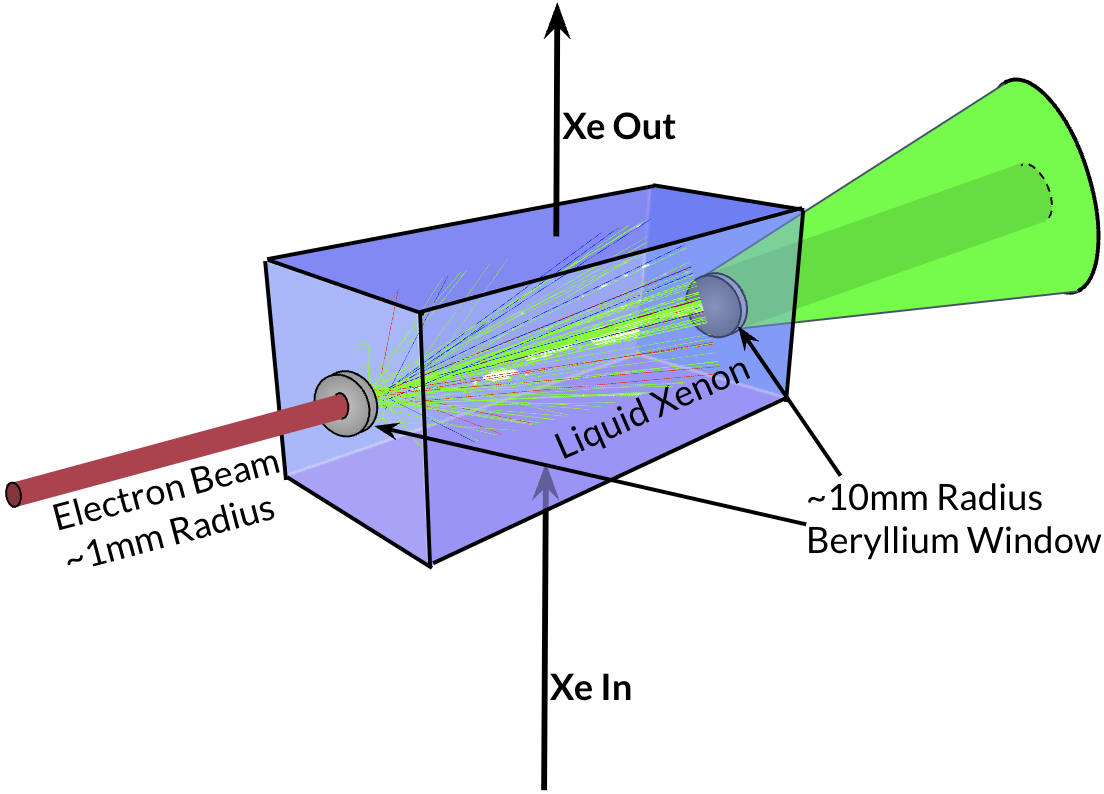
\includegraphics[width = \linewidth]{../images/Schematic4.png}
    \caption{\label{fig:schem}The liquid Xenon target setup. A 10 GeV electron beam is incident on the target from the left. The beam enters and exits the LXe target through a 10 mm diameter, 0.5 cm-thick Be window. The positrons exit the target and travel to the right.
    Fresh LXe is pumped vertically through the target chamber to replace the heated LXe.}
\end{figure}

\section{Simulation Results}
% start with fig 1 and describe phys setup
% discuss what physics was simulated in GEANT
% introduce previous work at FACET-II
% mention recognition of W targets but as long as normalizing by rad lengths that's all that matters 
% e- beam energy (10 GeV is F2 energy)
% cutoffs


% \subsection{Comparing Liquid Xenon and Tantalum Targets}
% discuss Hiroki's paper and why we are comparing to Ta
% state some form of prediction

% do sim on W target

% We compare our liquid Xenon target simulations in GEANT4 with simulations on Tantalum targets because FACET experience

% second fig
\begin{figure*}
    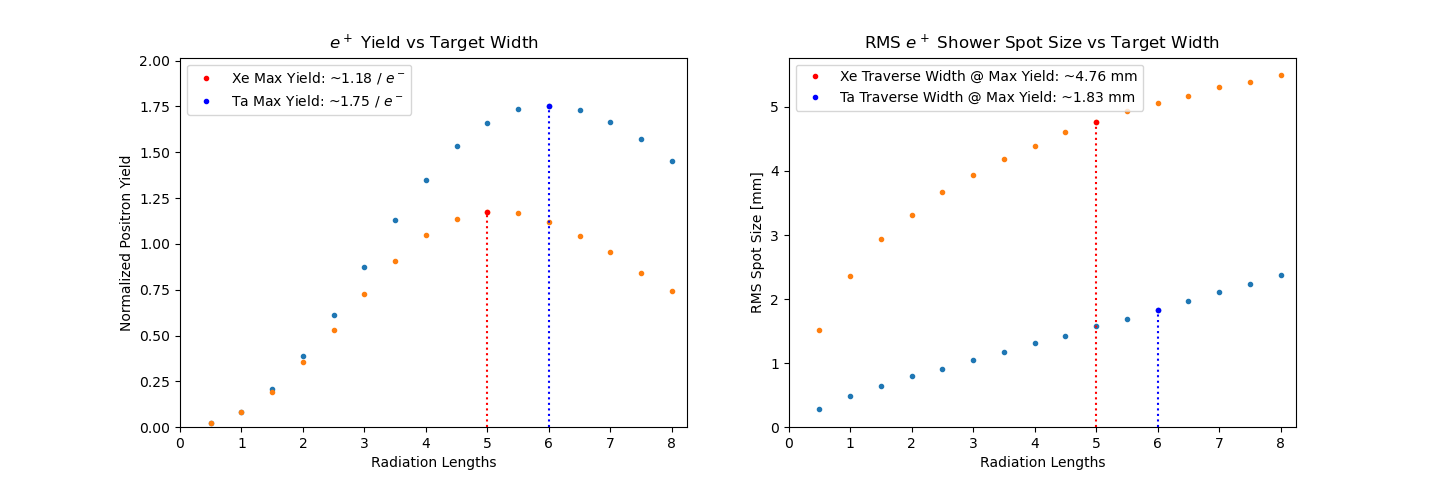
\includegraphics[width = \linewidth]{../images/CompYS.png}
    \caption{\label{fig:Yield} Positron yield and RMS transverse displacement upon exiting the target 
    per incident $e^-$ at 10 GeV.}
\end{figure*}

% Since we are familiar with Tantalum positron targets from~\cite{Fujii2019}, we decide to use Tantalum as a comparison
% to the liquid Xenon target in simulation. We use GEANT4~\cite{Geant4} to simulate the positron production for both targets.
Figure~\ref{fig:schem} illustrates the LXe target-beam interaction simulated using GEANT4~\cite{Geant4} G4EMStandardPhysics package to quantify positron production/beam parameters from the electromagnetic shower for both the LXe and Tantalum targets.  Previous studies at FACET-II considered a solid Tantalum (Ta) target, rather than the traditional tungsten (W) target, for positron generation~\cite{Fujii2019} which will serve as a useful comparison to the results of the LXe target.
% Using GEANT4~\cite{Geant4}, we compare our LXe target to a Tantalum (Ta) target due to previous
% experience with Tantalum positron targets at FACET-II
% We care more about similar results when normalizing by radiation lengths but recognize that WRe targets are common contenders for solid targets
% We note that tungsten is a more common target material and
% Ta was chosen

% maybe don't discuss 

\xout{Although tungsten (W) alloys are commonly used materials for conventional positron targets,we expect similar results for different solid target materials when normalizing by radiation lengths and therefore use Ta as a comparison.}

% We also simulated a Tungsten (W) target, but the results were similar enough to 
% Ta that we did not include it in the comparison.
% Since the electron beam energy is 10 GeV at FACET-II, an incident electron energy of 10 GeV was chosen for the simulations.
% We expect to see similar positron yields for both targets when normalizing by radiation lengths.
% Since the radiation length of liquid Xenon is around 7 times greater than that of Tantalum, 
% the transverse spread of the positron shower
% should be larger in the liquid Xenon target.  
The figures of merit used to compare the two targets are: 1) positron yield; 2) RMS spot size; and 3)energy deposition at the target.  For these comparisons, we only consider positrons at the exit of the target with an energy range of \textcolor{red}{2 MeV to 60 MeV and under 10 mm transverse displacement}, which is based off of similar positron acceptances in~\cite{Tang1995, Sheppard2003}.  Note that these cutoffs are for positrons just after exiting the target rather than at the end of a capture section of the accelerator.

\textcolor{red}{The figures are out of order numerically.}
% Comparison study between Tantalum (Ta) and liquid Xenon (LXe) because we have a reference study on Ta [].
% We used GEANT4 to simulate the collision between 10 GeV $e^-$ and a target.  We compare the results of using a
% Ta target and a LXe target.
% See Table~\ref{tab:G4Params} for parameters used in the simulation.
Table~\ref{tab:G4Params} shows the parameters used in the GEANT4 simulations.
\begin{table}[h]
    \centering
    \begin{tabular}{lcccc}
        \hline \hline
        \textbf{Material} & \textbf{Z} & \textbf{Density} [$\textrm{g} \cdot \textrm{cm}^{-3} $] & \textbf{Rad Length} [cm] \\
        \hline
        Tantalum (Ta) & 73 & 16.654 & 0.4094 \\
        % \hline
        Liquid Xe (LXe) & 54 & 2.953 & 2.872 \\
        \hline \hline
    \end{tabular}
    \caption{\label{tab:G4Params}Parameters used in GEANT4 simulation when comparing targets.}
\end{table}

% \subsubsection{Calculating Positron Emittance}
% \pagebreak
% To calculate the normalized RMS emittance of the positrons generated in pair production, 
% we utilize the following~\cite{Floettmann2003}
% \begin{subequations}
%     \begin{eqnarray}
%         \left\langle x^2 \right\rangle &= \frac{\sum x^2}{n} - \left( \frac{\sum x}{n} \right)^2, \label{subeq:x2} \\
%         \left\langle p_x^2 \right\rangle &= \frac{\sum p_x^2}{n} - \left( \frac{\sum p_x}{n} \right)^2, \label{subeq:p2} \\ 
%         \left\langle xp_x \right\rangle &= \frac{\sum xp_x}{n} - \frac{\sum x \sum p_x}{n^2}, \label{subeq:xp}
%     \end{eqnarray}
% \end{subequations}
% which gives us

% \begin{equation}
%     \varepsilon_{n,rms} = \frac{1}{m_0c}\sqrt[]{\left\langle x^2 \right\rangle \left\langle p_x^2 \right\rangle - \left\langle xp_x \right\rangle}. \label{eq:Emittance}
% \end{equation}
% Using this equation, we calculate the RMS emittance of the positrons for both Tantalum and liquid Xenon targets.  

% \begin{figure}[h]
%     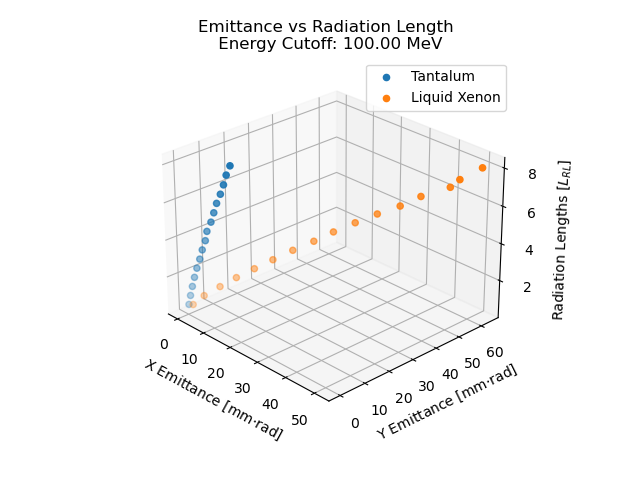
\includegraphics[width = .825\linewidth]{../images/CompEmittance.png}
%     \caption{\label{fig:Emittance}Normalized RMS positron emittance in a Tantalum and liquid Xenon target for differing target widths.
%     The positron energy cutoff was set to 100 MeV.}
% \end{figure}
% \begin{figure}[h]
%     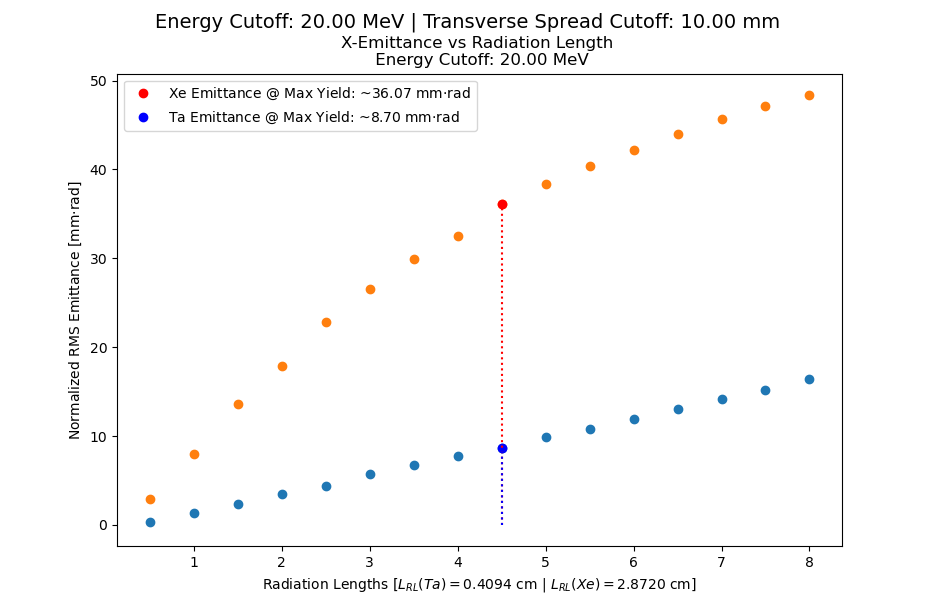
\includegraphics[width = \linewidth]{../images/XCompEmittance.png}
%     \caption{\label{fig:Emittance}RMS positron x-emittance in a Tantalum and liquid Xenon target for differing target widths.
%     The positron energy cutoff was set to 100 MeV.}
% \end{figure}
% \begin{figure}[h]
%     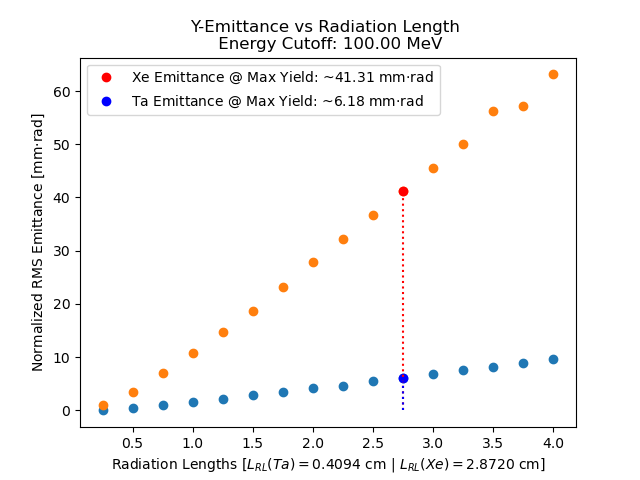
\includegraphics[width = \linewidth]{../images/YCompEmittance.png}
%     \caption{\label{fig:Emittance}RMS positron y-emittance in a Tantalum and liquid Xenon target for differing target widths.
%     The positron energy cutoff was set to 100 MeV.}
% \end{figure}

% \begin{figure*}[t]
%     \begin{subfigure}{\linewidth}
%         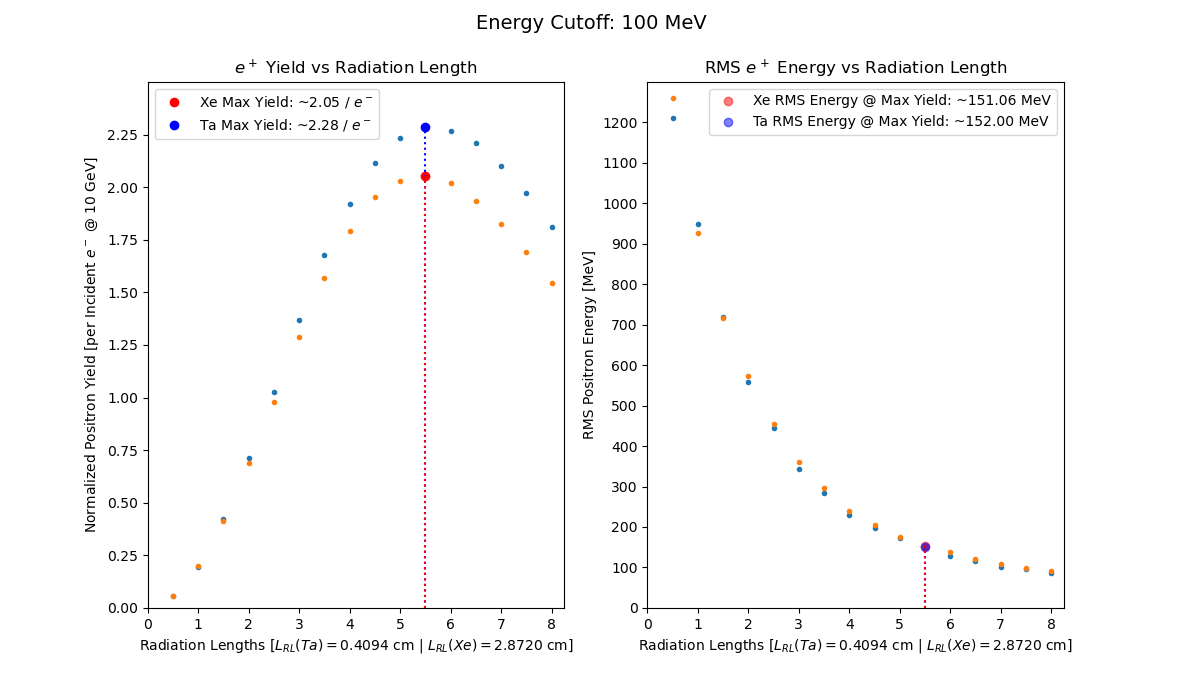
\includegraphics[width = .75\linewidth]{../images/CompYield.png}
%         \caption{\label{fig:Yield} Positron yield and energy at target exit.}
%         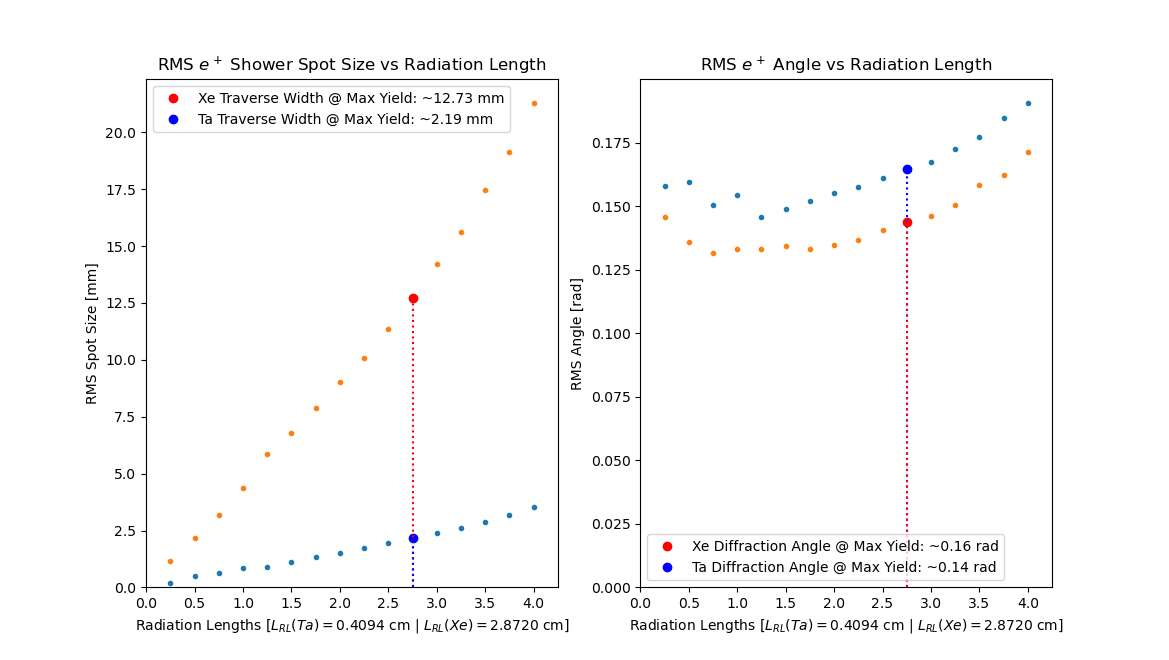
\includegraphics[width = .75\linewidth]{../images/CompATW.png}
%         \caption{\label{fig:ATW}Positron shower spot size and diffraction angle at the exit of the target.}
%     \end{subfigure}
%     \caption{\label{fig:Comps}Positron yield and RMS energy, 
%     shower spot size, and angular divergence of positrons upon exiting the target per incident $e^-$ at 10 GeV.}
% \end{figure*}

Figure~\ref{fig:Yield} displays positron yield and spot size as a function of radiation length for Ta and LXe.
\textcolor{red}{next sentence may change}
Although Figure~\ref{fig:Yield} indicates that the maximum positron yield occurs at a smaller radiation length for LXe compared to Ta,
the radiation length corresponding to maximum positron yield would be the same for both targets if we remove the energy and spot size cutoffs.
Observe that both targets generate a similar yield distribution when normalizing by
radiation lengths, as predicted.
The energy spectrum of the positrons exiting the
target are relatively equal for both target materials despite having different radiation lengths.

\textcolor{red}{At maximum positron yield, the transverse emittance for Ta
is $14\textrm{mm}\cdot\textrm{rad}$ while the transverse emittance for LXe is $33\textrm{mm}\cdot\textrm{rad}$.}
Even with a larger transverse emittance, the LXe emmittance is consistent with proposals at CLIC, NLC, and ILC~\cite{Tang1995, Seimiya2015, Vivoli2010}.
Ignoring our cuts in the data, the emittance and spot size for LXe is roughly 5 times larger than Ta, which can be attributed 
to their difference in radiation lengths.
% According to~\cite{Tang1995, Seimiya2015}, the transverse emittance for LXe is comparable for use in linear colliders.
% \begin{figure}[H]
%     \begin{subfigure}{\linewidth}
%         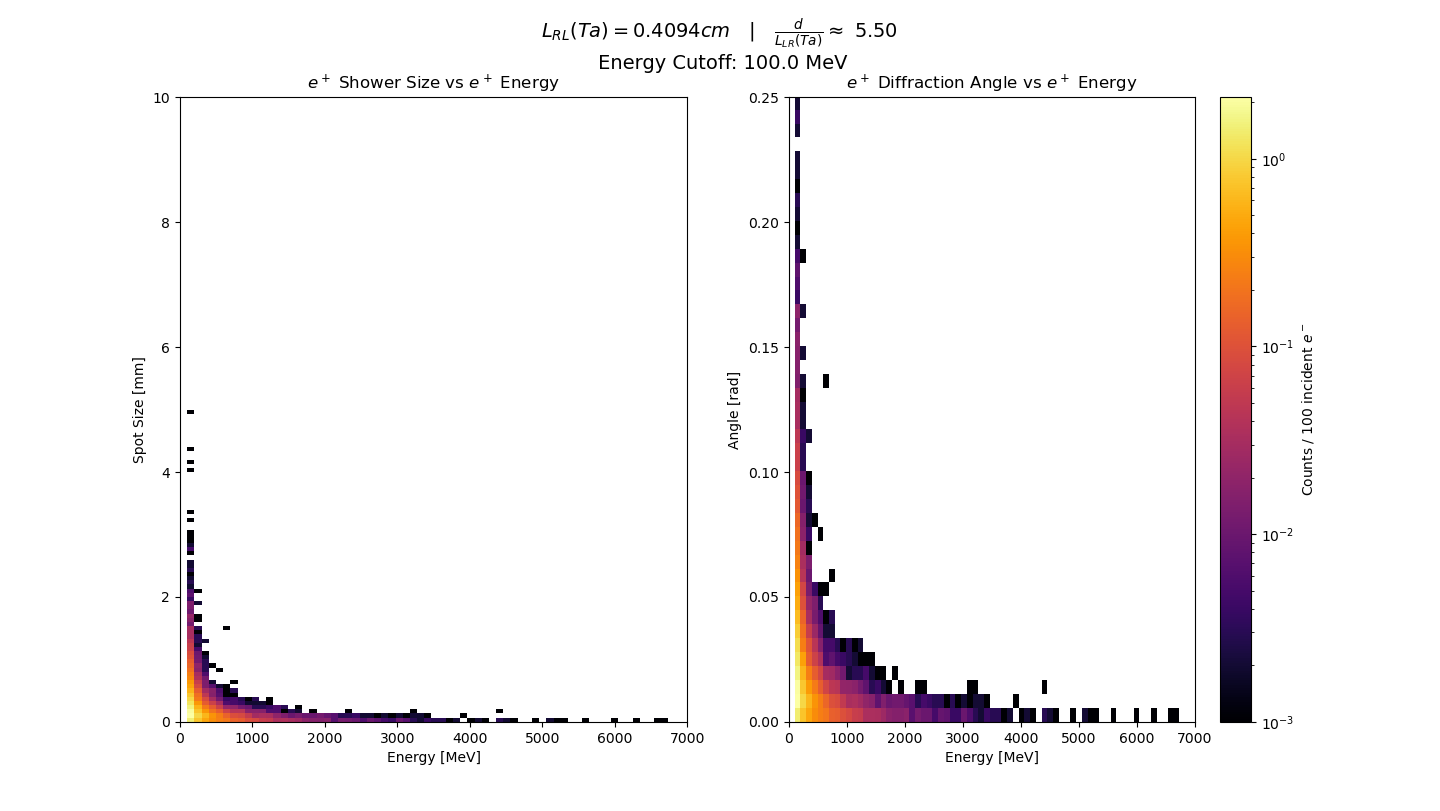
\includegraphics[width = \linewidth]{../images/TaHists.png}
%         \caption{\label{fig:TaHists}Tantalum target.}
%         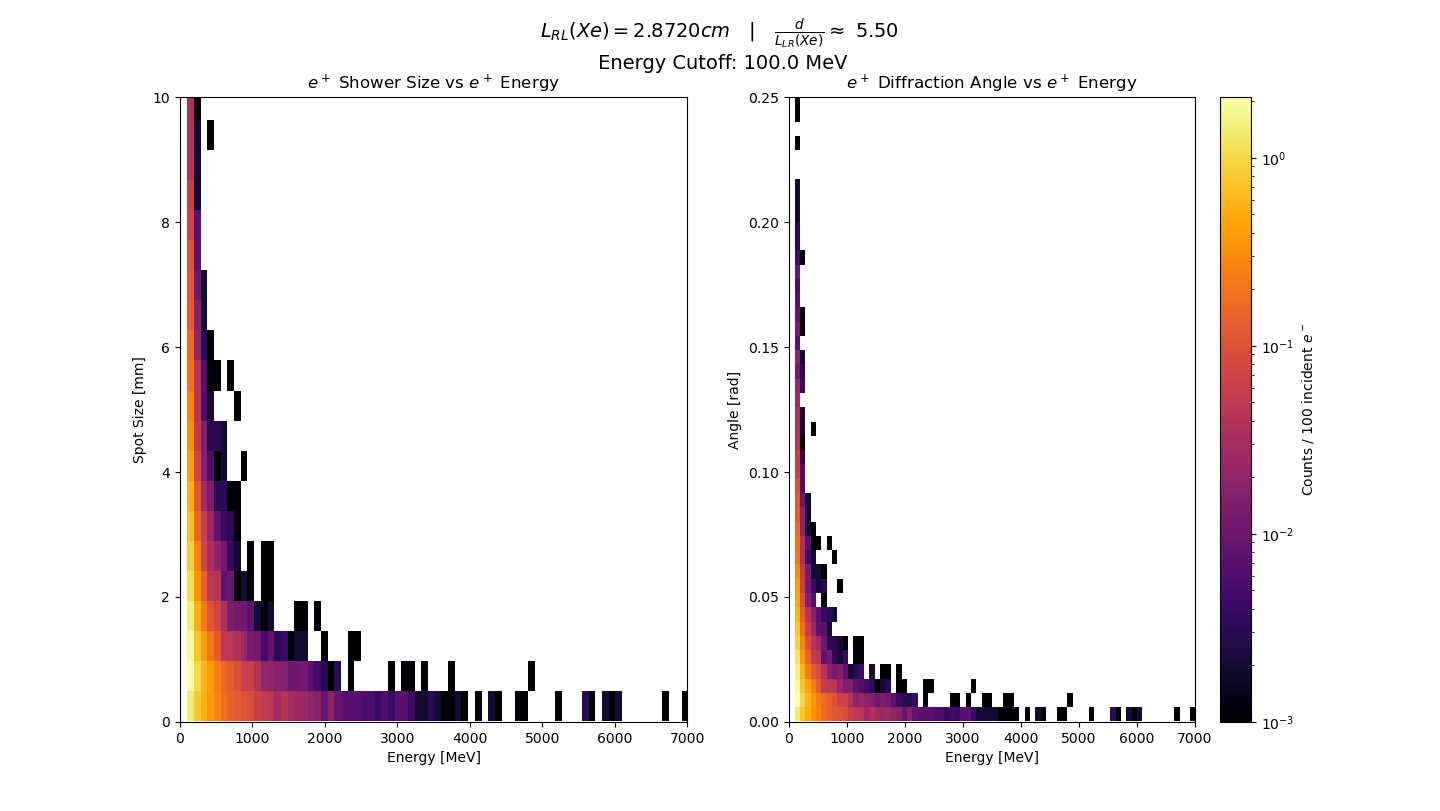
\includegraphics[width = \linewidth]{../images/XeHists.png}
%         \caption{\label{fig:XeHists}Liquid Xenon target.}
%     \end{subfigure}
%     \caption{\label{fig:Hists}Transverse displacement and angular diffraction of positrons as a function
%     of their energy upon target exit.  Data is shown for widths of 4.5 radiation lengths (max $e^+$ yield).}
% \end{figure}
Despite both having the same angular divergence, the difference in radiation lengths is great enough that we find a larger 
RMS spot size for LXe compared to Ta in Figure~\ref{fig:Yield} even with our cuts in place.
% Although we found the angular divergence of the positrons exiting the target to be similar for both materials,
% Figure~\ref{fig:Yield} indicates that the transverse displacements are larger for the LXe target.  
% This can be explained by the fact that the radiation length of LXe is roughly seven times that of Tantalum.

% \begin{figure}[H]
%     \centering
%     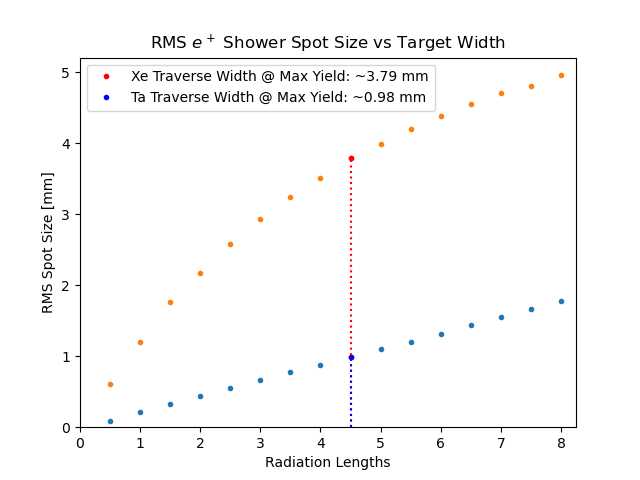
\includegraphics[width = \linewidth]{../images/CompTW.png}
%     \caption{\label{fig:TW}Transverse displacement of positrons as a function of radiation length.}
% \end{figure}

% Notice that in Figure~\ref{fig:TW}, the angular divergence of positrons is roughly the same for both targets,
% yet the transverse widths are more broadly distributed for the liquid Xenon target.  This can be explained by the 
% fact that the radiation length of LXe is roughly seven times that of Tantalum.
We extract energy deposited in the target from the simulations which is a critical component of our flow calculations in the following section.
Figure~\ref{fig:EDep} compares the energy deposited in the target for each material per incident $e^-$.
As we indicate in Section~\ref{sub:Flow}, the flow of LXe accounts for the energy deposit.  
It is clear from Figure~\ref{fig:EDep} that both targets follow the same energy deposition distribution as a function of radiation length.

\begin{table*}
    \centering
    \begin{tabular}{lccccc}
        \hline \hline
        \textbf{Parameter} & \textbf{Unit} & \textbf{FACET-II}~\cite{FACET2016} & \textbf{ILC}~\cite{Nagoshi2020} & \textbf{C$^3$}~\cite{Bai2021} & \textbf{Optimal} \\
        \hline
        Energy & GeV & 10 & 3 & 3 & 10 \\
        $e^-$/bunch & $10^{10}$ & 1.25 & 2.5 & 0.78 & 1.125 \\
        Bunches/train & & 1 & 1312 & 133 & 1000 \\
        Rep. rate & Hz & 10 & 5 & 120 & 11.10 \\
        PEDD/train & $\textrm{J}\cdot\textrm{g}^{-1}$ & 0.107 & 84.0 & 2.66 & 96.1 \\
        Flow rate & $\textrm{L}\cdot\textrm{s}^{-1}$ & 0.0049 & 0.073 & 1.75 & 0.16 \\
    \hline \hline
    \textbf{Beryllium Window} \\
        $E_{\textrm{dep}}$/bunch train & J &  0.014 & 10.65 & 0.34 & 12.18 \\
        Temperature change & K$\cdot \textrm{s}^{-1}$ & 2.56 & 1009 & 766 & 2560 \\
    \hline \hline
    \end{tabular}
    \caption{\label{tab:BeamInfo}Electron beam parameters and associated target quantities for FACET-II, ILC, C$^3$, and the optimal beam setup.
    The Beryllium window quantities are specific to a 10mm radius, 0.5 mm-thick Be disk.  Note that the window parameters
    correspond to the exit window only since the entrance window receives a significantly smaller energy deposit per incident $e^-$.}
\end{table*}

\begin{figure}[H]
    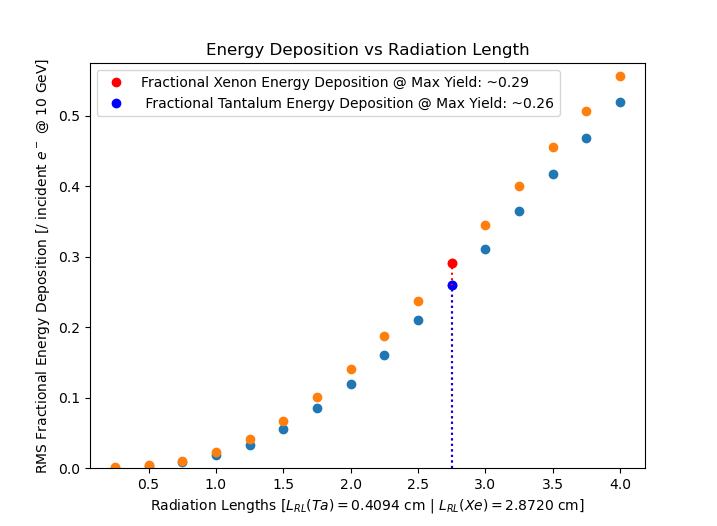
\includegraphics[width = \linewidth]{../images/CompDeps.png}
    \caption{\label{fig:EDep}RMS fractional energy deposition in Ta and LXe targets per incident electron at 10 GeV.}
\end{figure}

% \subsection{Setting a Cutoff Traverse Width}
% Although the max yield for liquid Xenon is on par with that of the Tantalum target
% according to Figure~\ref{fig:Yield}, the physical spread of positrons produced
% from the liquid Xenon target is much larger than that of the Tantalum target (Figure~\ref{fig:Hists}).
% As a result, only a
% fraction of the positrons that exit the target will have the right characteristics to make it down the rest of
% the accelerator.  In order to accurately assess the plausibility of using a liquid Xenon positron target,
% we set cutoffs for the traverse width of positrons created during the collision.

% \begin{figure}[H]
%     \begin{subfigure}{.45\textwidth}
%         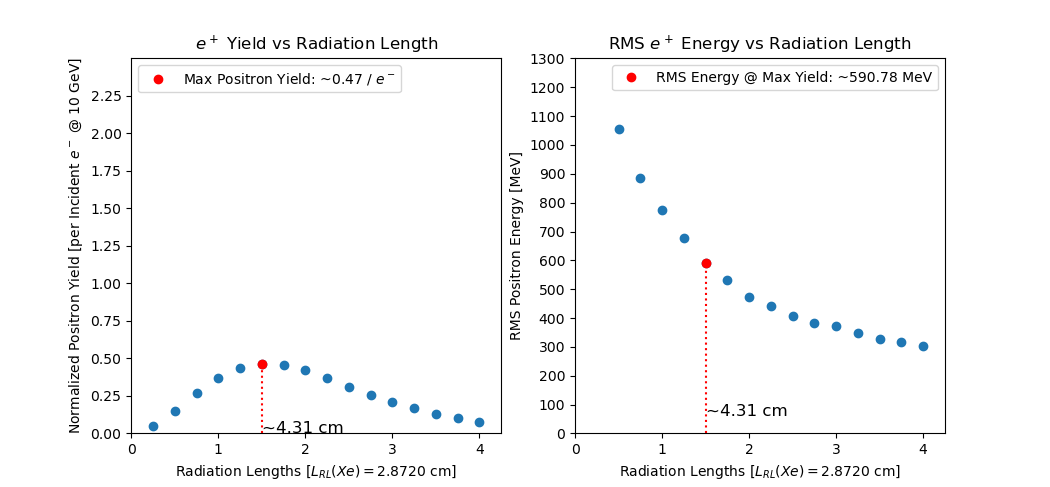
\includegraphics[height = .5\linewidth]{../images/XeYield1mmCutoff.png}
%         \caption{\label{fig:XeY1}1 mm cutoff}
%         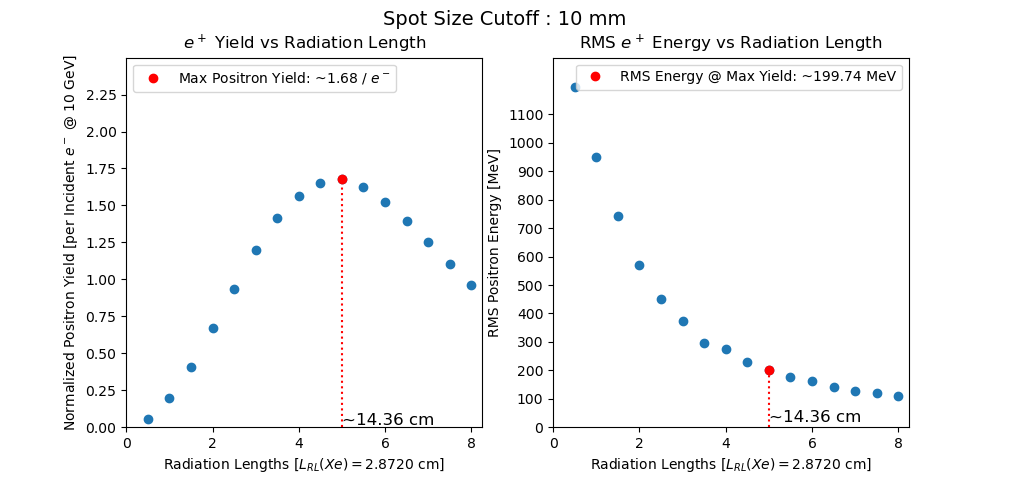
\includegraphics[height = .5\linewidth]{../images/XeYield10mmCutoff.png}
%         \caption{\label{fig:XeY5}10 mm cutoff}
%     \end{subfigure}
%     \caption{\label{fig:YieldCut}Positron yield and energy using 
%     a liquid Xenon target with a 1 mm and 10 mm traverse width cutoff.}
% \end{figure}

% \begin{figure}[H]
%     \begin{subfigure}{.5\textwidth}
%         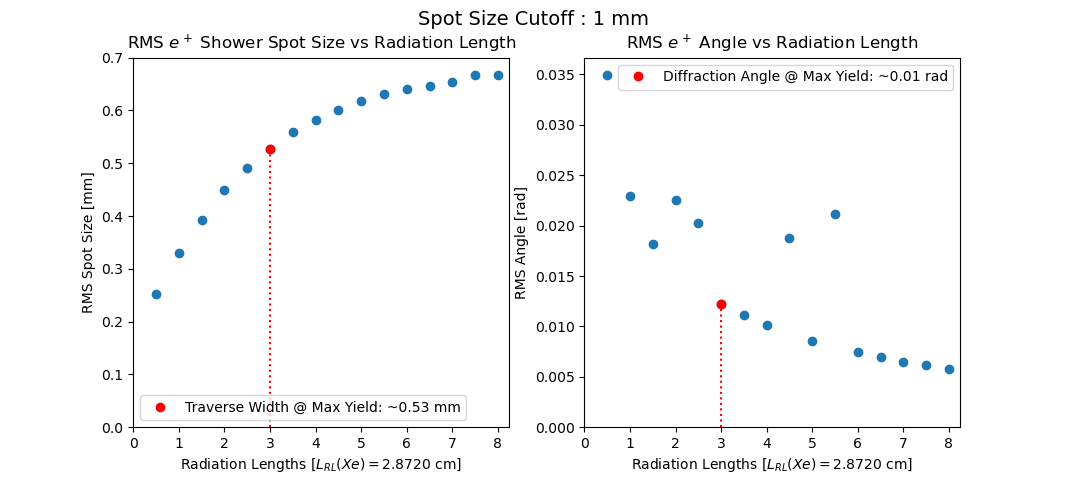
\includegraphics[height = .45\linewidth]{../images/XeATW1mmCutoff.png}
%         \caption{\label{fig:XeATW1}1 mm cutoff}
%         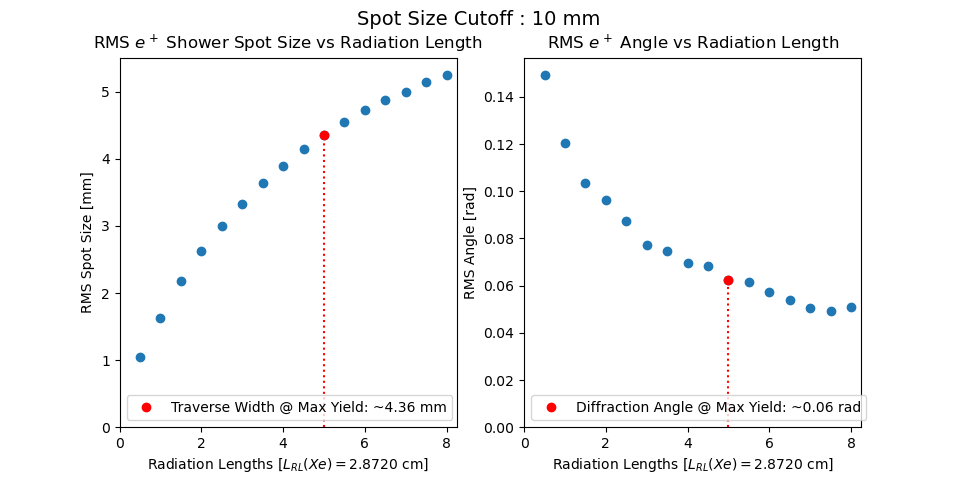
\includegraphics[height = .5\linewidth]{../images/XeATW10mmCutoff.png}
%         \caption{\label{fig:XeATW5}10 mm cutoff}
%     \end{subfigure}
%     \caption{\label{fig:ATWCut}Positron spot size and angular diffraction using 
%     a liquid Xenon target with a 1 mm and 10 mm traverse width cutoff.}
% \end{figure}
% It is reassuring to see that even after removing the positrons from the dataset 
% with large transverse distances from the beam path, there are still a comparable number
% of positrons that we predict will be able to make it to the next stage of the accelerator [].

\section{Energy Depositions and Flow Considerations for LXe}
% what are we trying to achieve
% trying to figure out for different parameters how much Edep and how to deal with it

\subsection{Calculating the LXe Flow Rate} \label{sub:Flow}
% To obtain the flow rate of the LXe, we first note preliminary 
% values using the information given in Table~\ref{tab:XeInfo}.
% To see beam parameter sets and resultant quantities, seek Table~\ref{tab:BeamInfo}.

% \begin{table}[H]
%     \centering
%     \begin{tabular}{lccc}
%         \hline \hline
%         \textbf{Liquid Xenon} & \textbf{Symbol} & \textbf{Value} & \textbf{Unit} \\
%         % Quantity & Symbol & Value & Units \\
%         % \hline
%         % $\textrm{g}\cdot\textrm{mol}^{-1}$
%         Molar Mass & M & 131.293 & u \\
%         Density & $\rho$ & 2.953 & $\textrm{g} \cdot \textrm{cm}^{-3}$ \\
%         Vapor Pressure & $p$ & 300 & kPa \\
%         Heat of Vaporization & $\Delta \textrm{H}$ & 12.636 & kJ$\cdot$mol$^{-1}$ \\
%         Heat of Vap./Volume & $\Delta \textrm{H}_{\textrm{vol}}$ & 284.205 & J$\cdot \textrm{cm}^{-3}$ \\
%         Radiation Length & $\textrm{L}_{\textrm{RL}}$ & 2.872 & cm \\
%         Width & $\frac{\textrm{d}}{\textrm{L}_{\textrm{RL}}}$ & 4.5 & $\textrm{L}_{\textrm{RL}}$ \\
%         % Volume & V & & cm$^3$ \\
%         \hline \hline
%     \end{tabular}
%     \caption{\label{tab:XeInfo}LXe material and target properties.}
% \end{table}

For our calculations, we assumed a spot size of 6 mm 
radius which was determined by the shower size.  This resulted in a volume of 14.6 cm$^3$ of LXe interacting with the beam shower.
By using heat of vaporization, we determined the energy required to vaporize the LXe.
PEDD is calculated by considering the energy deposit per bunch train and the mass of the interacting volume of LXe (43.16 g).
Note that some of the PEDD values in Table~\ref{tab:BeamInfo} far exceed the typical maximum PEDD of 35 $\textrm{J}\cdot\textrm{g}^{-1}$ for solid targets~\cite{Seimiya2015}.
Since the LXe is constantly circulating in the target, the PEDD is not a limiting factor for the LXe target.
By using the bunch train energy deposits and beam repetition rates along with the amount of energy required to vaporize LXe for a given volume (calculated to be 284.205 J$\cdot \textrm{cm}^{-3}$),
the time required to vaporize the 14.6 cm$^3$ of LXe was obtained.
We based the LXe flow rates off of the time evacuate the volume before the next bunch train
arrival at the target.

\textcolor{red}{Subject to change.}\\
When considering the optimal beam parameters for the LXe target, we assumed a delivery rate of $10^{14}$ ${e^+\cdot \textrm{s}^{-1}}$
to the IP.  We also assumed a safety factor of 1.5 positrons after the target which gave a positron yield of 1.2 per incident electron.
Lastly, we took the drive bunch energy to be 10 GeV and the energy deposition to be 2.3 GeV/$e^-$, which was based off of the simulation results.
From these assumptions, we chose the beam parameters that brought the energy deposit per bunch train closest to the energy required to 
vaporize the LXe.


% \begin{table*}
%     \centering
%     \begin{tabular}{lcccc}
%         \hline \hline
%         \textbf{Beam Parameters} & \textbf{Symbol} & \textbf{FACET-II}~\cite{FACET2016} & \textbf{ILC}~\cite{Seimiya2015} & \textbf{Units} \\
%         \hline
%         Energy & $E$ & 10.0 & 6.0 & GeV \\
%         Repetition Rate & $f$ & 10 & 300 & Hz \\
%         Charge & $q$ & 2 & 3.204 & nC \\
%         Number of $e^-$ & n & 1.248 & 2.0 & $10^{10}$ \\
%         \hline \hline
%         \textbf{Resultant Quantities} \\
%         \hline
%         Energy Deposition/$e^-$ & E$_{\textrm{dep}}$ & 1.9 & & GeV \\
%         Energy Deposit/Pulse & $\epsilon$ & 3.8 & 482.1 & J \\
%         Peak Energy Deposit Density & $\epsilon_\rho$ & $1.96\times 10^{-2}$ & 15.22 & J$\cdot\textrm{g}^{-1}$ \\
%         Power Deposit/Pulse & $P_\textrm{dep}$ & $38.0$ & $1.45\times 10^5$ & W \\
%         Flow Rate due to Vaporization & Q & $0.134$ & 508.9 & cm$^3\cdot \textrm{s}^{-1}$ \\
%         Main Shower Path Flow Rate & $Q_\textrm{vol}$ & 0.5170 & 15.51 & L$\cdot \textrm{s}^{-1}$ \\
%         \hline \hline
%     \end{tabular}
%     \caption{\label{tab:BeamInfo}Electron beam parameters and associated target quantities for ILC and FACET-II.}
% \end{table*}

% We first convert the heat of vaporization to units of energy per unit volume (J$\cdot \textrm{cm}^{-3}$),
% \begin{equation}
%     \Delta \textrm{H}_\textrm{vol} = \frac{\Delta \textrm{H}\cdot \rho}{\textrm{M}}. \label{eq:HoV}
% \end{equation}
% Then, one can calculate the number of electrons per beam bunch, by comparing the 
% total charge of the beam bunch to the charge of an electron
% ($e \approx 1.602 \times 10^{-10}$ nC).
% % , as follows from Eq.~(\ref{subeq:n}).
% From this, we calculate the total energy deposited in the LXe target.
% Lastly, we obtain the flow rate of LXe required to replace the vaporized Xenon due
% to the energy deposited by the beam,
% \begin{equation}
%     Q = \frac{\epsilon \cdot f}{\Delta \textrm{H}_{\textrm{vol}}}.
% \label{eq:Q}
% \end{equation}
% % as seen in Eq.~(\ref{subeq:Etot}).
% % \begin{subequations}
% %     \begin{eqnarray}
% %         \Delta \textrm{H}_\textrm{vol} &=& \frac{\Delta \textrm{H}\cdot \rho}{\textrm{M}}, \label{subeq:HoV} \\
% %         n &=& \frac{q}{e}, \label{subeq:n} \\
% %         \epsilon &=& n \cdot E_{\textrm{dep}} \label{subeq:Etot}.
% %     \end{eqnarray}
% % \end{subequations}
    

% In case one wants to calculate the flow rate required to move the entire volume encompassing the main
% part of the EM shower, the volume can be approximated by a rectangular prism with 
% side lengths equal to the diameter of the Beryllium windows (see next section) and width equal to the target width.  
% At max positron yield, this gives 
% ${\textrm{V} = (2 \textrm{ cm})^2 \cdot 4.5\textrm{L}_{\textrm{RL}} \approx 51.70 \textrm{ cm}^3}$.
% As a result, the required flow rate to move volume V in the amount of time between beam pulses is
% shown in Table~\ref{tab:BeamInfo} as $Q_\textrm{vol}$.

\subsection{Beryllium Windows for the Target Chamber}

% \begin{table}[H]
%     \centering
%     \begin{tabular}{lccc}
%         \hline \hline
%         \textbf{Be Quantity} & \textbf{Symbol} & \textbf{Value} & \textbf{Unit} \\
%         \hline
%         % Atomic Number & Z & 4 & \\
%         % Density & $\rho$ & 1.844 & g$\cdot$cm$^{-3}$ \\
%         Rupture Modulus & $F_a$ & 400 & MPa \\
%         Specific Heat & $c_p$ & 1.82 & J$\cdot$g$^{-1}\cdot$K$^{-1}$ \\
%         % Yield Strength & $\sigma_\textrm{y}$ & 240 & MPa \\
%         % Tensile Strength & $\sigma_\textrm{t}$ & 370 & MPa \\
%         % Shear Strength & $\sigma$ & 1234 & MPa \\
%         % Thermal Conductivity & $\kappa$ & 216 & W$\cdot$m$^{-1}$$\cdot$K$^{-1}$ \\
%         % \hline \hline
%         % \textbf{Quantities} \\
%         % \hline
%         % Height
%         % % \footnote{Difference in height between the Beryllium window and the top of the liquid Xenon chamber.} 
%         % & $h$ & 1.0 & m \\
%         Radius & $r$ & 10.00 & mm \\
%         % Contact Area & $A$ & $100\pi$ & mm$^2$ \\
%         Pressure & $P$ & 329 & kPa \\ % 328.968
%         % Force & $F$ & 9.100 & N \\
%         Safety Factor & $S_F$ & 4 \\
%         Empirical Constant & $K$ & 0.75 \\
%         Thickness & $T$ & 0.5 & cm \\ % 496.701
%         \\
%         $E_{\textrm{dep}}$/Bunch Train & $E^{\prime}_{\textrm{dep}}$ & \begin{tabular}{@{}c@{}} 0.01 (F) \\ 9.46 (ILC) \\ 0.30 (C$^3$) \\ 13.8 (O) \end{tabular} & J \\
%         \\
%         Temperature Change & $\Delta T$ & \begin{tabular}{@{}c@{}} 0.912 (F) \\ 359 (ILC) \\ 0.27 (C$^3$) \\ 883 (O) \end{tabular} & K$\cdot \textrm{s}^{-1}$ \\
%         \hline \hline
%     \end{tabular}
%     \caption{\label{tab:BeInfo}Useful quantities and properties of solid Beryllium.
%     The quantities are specific to a 10mm radius Beryllium disk.  "F" denotes FACET-II
%     parameters and similarly "O" for optimal parameters.  $E^{\prime}_{\textrm{dep}}$
%     and $\Delta T$ correspond to the exit window only since the entrance window recieves
%     a negligible energy deposit per incident $e^-$.}
% \end{table}
We explore using Beryllium (Be) windows for the beam to enter and exit the target chamber.
The pressure on the Be windows is dominated by the vapor pressure of LXe which is around 300 kPa.
% Utilizing Bernoulli's equation for conservative fields and the fact that the flow rate for the LXe can be quite small (Table~\ref{tab:BeamInfo}),
% we can approximate the pressure on a Be window to be roughly 329 kPa.
% , which is of the form
% \begin{equation}
%     P = \frac{1}{2} \rho v^2 + \rho g h + p,
% \label{eq:Bern}
% \end{equation}
% where $v$ is the fluid flow rate, $g$ is acceleration due to gravity, $h$ is the height of the Xenon chamber
% relative to the height of the window,
% and $p$ is the additional external pressure (in this case $p$ refers to the vapor pressure of LXe $\sim 300 \textrm{kPa}$).
% However, as seen in Table~\ref{tab:BeamInfo}, the flow rate for the LXe can be quite small,
% so we can approximate the pressure to be
% Additionally, the liquid Xenon chamber is in vacuum, and we are comparing differences in total pressures,
% so we can ignore $p$ as well.  
% \begin{equation}
%     P = \rho g h + p,
%     \label{eq:BernSimp}
% \end{equation}
% where $g$ is acceleration due to gravity, $h$ is the height of the target chamber
% relative to the height of the window,
% and $p$ is the additional pressure (in this case $p$ refers to the vapor pressure of LXe $\sim 300 \textrm{kPa}$~\cite{Mount2017}).
% From Eq.~(\ref{eq:BernSimp}), we can calculate the force on a Be window.
% : $F = P\cdot A$.
% In order to determine the required thickness of the windows, we utilize methods described in~\cite{Crystran2019}.
% First we calculate a constant related to the safety factor of our thickness, which takes into account
% the method with which the Be window is inserted into the target chamber.
% An empirical constant $K = 0.75$ is chosen if the window is clamped into the target chamber, and
% $K = 1.125$ if the window is unclamped in the target chamber.  For a given safety factor,
% we have a thickness of
% \begin{equation}
%     T = r\cdot\sqrt{\frac{S_F\cdot K\cdot P}{F_a}}.
% \end{equation}
Reference~\cite{Crystran2019} provides a method to calculate the required thickness of the Be windows, which we found to be 0.5 mm.
% From this method, we get a required thickness of 0.5 cm.
Using this thickness, we simulated the energy deposited in the Be windows and found that
the energy deposited in the entrance window is on the order of $10^{-1}$ MeV/incident~$e^-$ and the exit window
on the order of 6 MeV/incident~$e^-$.  
According to the conclusions of~\cite{Ammigan2019},
the temperature shocks corresponding to the energy deposits in the windows is of negligible concern at 
FACET-II.  However, we would expect to see microcracks in the exit window for ILC and C$^3$.
Note that the melting point of Beryllium is 1285 $^{\circ}$C, so the temperature change corresponding to the optimal
beam parameters requires attention.
% For an optimal and/or ILC-type collider, the exit window runs the risk of melting.

%~\ref{fig:WinDeps}.

% \begin{figure}[H]
%     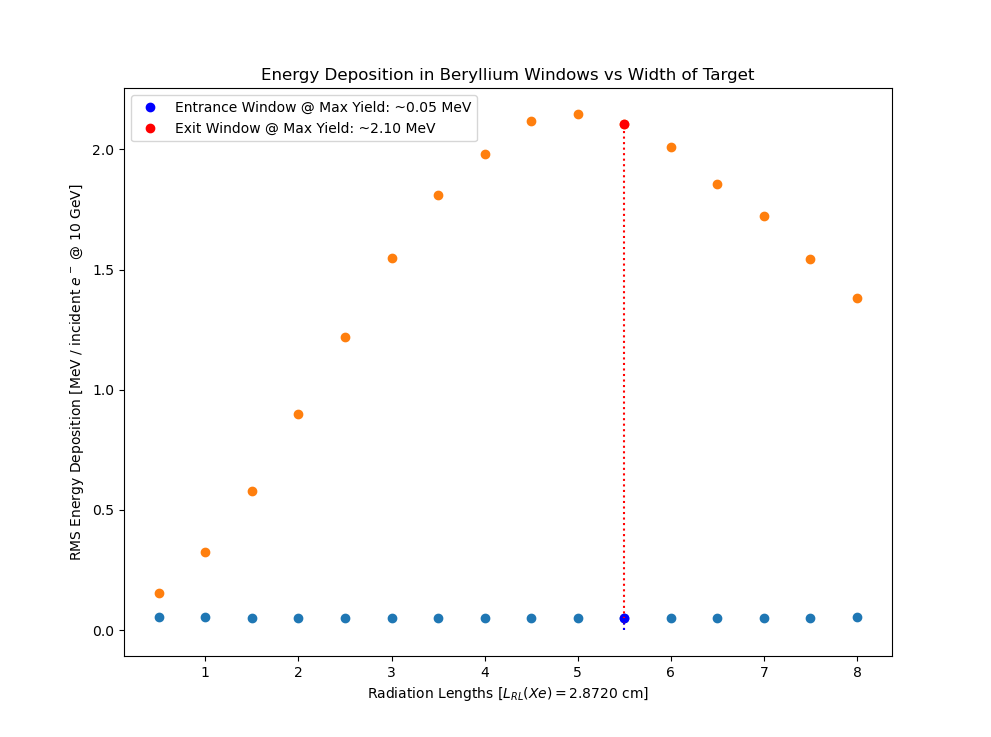
\includegraphics[width = .5\textwidth]{../images/WindowDeps.png}
%     \caption{\label{fig:WinDeps}Energy deposition on incident and exit Beryllium windows per incident $e^-$.}
% \end{figure}
% As depicted in Figure 
%~\ref{fig:WinDeps}
% , the energy deposited in both Beryllium windows is of no concern?
% \textbf{TODO}
% Explore how much heat Be windows can take in given amount of time like done above for LXe??
% Energy transfer from windows to LXe??

\section{Conclusion}
Through GEANT4 simulations, we determined that a LXe $e^+$ target produces comparable yields to its solid target counterparts.
The benefit of using a LXe target is that it does not deteriorate over time as compared to solid targets which require replacement due to degradation.
Despite the slight discrepancies in $e^+$ spread between solid targets and LXe, the apparent benefits of using a LXe target outweighs this disadvantage.
The most important considerations while building a LXe apparatus would be accounting for the pressure of the Xenon and the corresponding flow rates.  Using Be windows for the beam entrance and exit of the LXe target chamber have minimal affect on the beam quality output according to simulations, and should be considered for use when designing a LXe target.
Note that for certain beam parameters the Be windows may not be well-suited for the high temperature changes.
In such cases, additional considerations should be made for the target windows.
Further exploration of LXe positron target could entail more detailed simulations of the beam interaction with the LXe,
% more detailed materials simulations
such as cavitation bubbles and turbulent flows, as well as simulating a capture system on the exit of the target.
It may also be useful to determine the energy deposit in the LXe as a function of target depth to better approximate flow rates.
% Additional considerations for target windows should be made for optimal and ILC-type linear colliders.
% We believe that the parameter sets we developed for the LXe target make it suitable for future linear collider applications.
Source code and sample data from GEANT4 simulations can be found at 
\url{https://github.com/MaxVarverakis/LiquidXenonSims.git}.










% \begin{acknowledgments}
% We wish to acknowledge the support of the author community in using
% REV\TeX{}, offering suggestions and encouragement, testing new versions,
% \dots.
% \end{acknowledgments}

% \appendix
% \section{Appendixes}

% To start the appendixes, use the \verb+\appendix+ command.
% This signals that all following section commands refer to appendixes
% instead of regular sections. Therefore, the \verb+\appendix+ command
% should be used only once---to setup the section commands to act as
% appendixes. Thereafter normal section commands are used. The heading
% for a section can be left empty. For example,
% \begin{verbatim}
% \appendix
% \section{}
% \end{verbatim}
% will produce an appendix heading that says ``APPENDIX A'' and
% \begin{verbatim}
% \appendix
% \section{Background}
% \end{verbatim}
% will produce an appendix heading that says ``APPENDIX A: BACKGROUND''
% (note that the colon is set automatically).

% If there is only one appendix, then the letter ``A'' should not
% appear. This is suppressed by using the star version of the appendix
% command (\verb+\appendix*+ in the place of \verb+\appendix+).

% \section{A little more on appendixes}

% Observe that this appendix was started by using
% \begin{verbatim}
% \section{A little more on appendixes}
% \end{verbatim}

% Note the equation number in an appendix:
% \begin{equation}
% E=mc^2.
% \end{equation}

% \subsection{\label{app:subsec}A subsection in an appendix}

% You can use a subsection or subsubsection in an appendix. Note the
% numbering: we are now in Appendix~\ref{app:subsec}.

% Note the equation numbers in this appendix, produced with the
% subequations environment:
% \begin{subequations}
% \begin{eqnarray}
% E&=&mc, \label{appa}
% \\
% E&=&mc^2, \label{appb}
% \\
% E&\agt& mc^3. \label{appc}
% \end{eqnarray}
% \end{subequations}
% They turn out to be Eqs.~(\ref{appa}), (\ref{appb}), and (\ref{appc}).

% % The \nocite command causes all entries in a bibliography to be printed out
% % whether or not they are actually referenced in the text. This is appropriate
% % for the sample file to show the different styles of references, but authors
% % most likely will not want to use it.
% \nocite{*}

\bibliography{LqdXePositronTarget}% Produces the bibliography via BibTeX.

\end{document}
%
% ****** End of file apssamp.tex ******
